We first analyze the Andronov-Hopf bifurcation occurring for a system with one parameter $\alpha$ in a two-dimensional state space having:
\begin{align*}
    \dot{x_1} = \alpha x_1 - x_2 - x_1(x_{1}^{2}+x_{2}^{2}) \\
    \dot{x_2} = x_1 + \alpha x_2 - x_2(x_{1}^{2}+x_{2}^{2})
\end{align*}
% Visualize the bifurcation of the system by plotting three phase diagrams.
We plot three phase diagrams of the bifurcation with different values for $\alpha$ as reported in the table underneath (table \ref{tab:task3_phase_diagrams}): 

\renewcommand{\arraystretch}{1.5} % Adjust vertical spacing in the table
\begin{table}[H]
    \centering
    \begin{tabular}{|c|>{\centering\arraybackslash}m{0.4\textwidth}|>{\centering\arraybackslash}m{0.3\textwidth}|}
    %\begin{tabular}{|c|c|c|}
    \hline
    \textbf{Value of $\alpha$} & \textbf{Visualization of the Phase Diagram} & \textbf{Observations} \\
    \hline
    -1 & 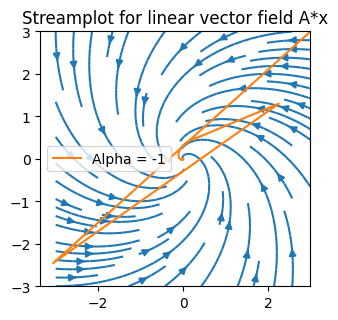
\includegraphics[width=0.31\textwidth]{images/task3/A-H_bifurcation_-1.png} & 
    Trajectories spiral inward around the equilibrium at the origin. 
    The equilibrium is asymptotically stable. \\
    \hline
    0 & 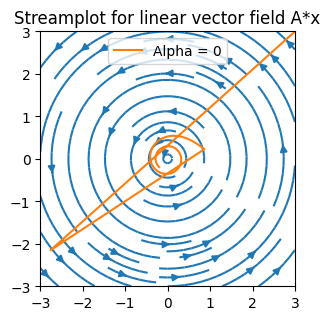
\includegraphics[width=0.31\textwidth]{images/task3/A-H_bifurcation_0.png} & 
    Trajectories neither converge nor diverge. 
    They form loops around the equilibrium at the origin.
    The equilibrium is asymptotically "weakly" stable.\\
    \hline
    1 & 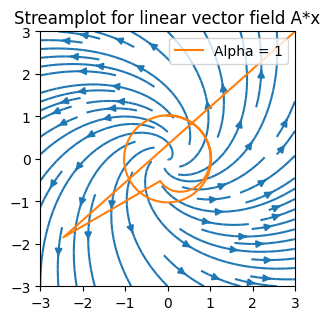
\includegraphics[width=0.31\textwidth]{images/task3/A-H_bifurcation_1.png} & Trajectories spiral outward and diverge from the equilibrium at the origin. The system is unstable.\\
    \hline
    \end{tabular}
    \caption{Observations of Phase Diagrams for Different $\alpha$ Values}
    \label{tab:task3_phase_diagrams}
\end{table}

% For α = 1, numerically compute and visualize two orbits of the system (8).
Let's now visualize two orbits of the system, for $\alpha=1$ forward in time, one starting at the
point $(2, 0)$ and the other at $(0.5, 0)$. To do so, we used Euler’s method with a step size 10 times smaller by defining the time range as \texttt{time = np.linspace(0, 100, 10000)} instead of \texttt{np.linspace(0, 10, 100)}.
\begin{figure} [H]
    \centering
    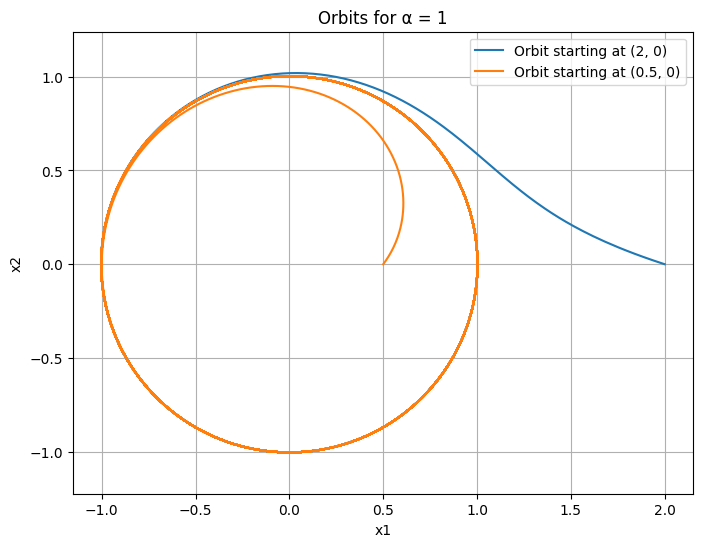
\includegraphics[width=0.45\textwidth]{images/task3/orbits.png}
    \caption{Two orbits of the system with $\alpha=0$ for 2 different origins}
    \label{fig:task3_orbits}
\end{figure}

    %add observations / comments !


% Visualize the bifurcation surface of the cusp bifurcation (9) in a 3D plot.
The cusp bifurcation occurs for a system with two parameters $\alpha=(\alpha_1, \alpha_2)$ in a one-dimensional state space having:
\begin{align*}
    \dot{x} = \alpha_1 + \alpha_2 x - x^3
\end{align*}
We visualize the bifurcation surface (i.e. all points $(x, \alpha_1, \alpha_2)$ where $\dot{x} = 0$) in a 3D plot with $\alpha_1$ and $\alpha_2$ on the bottom plane and $x$ in the third direction. To do so we  sample points $(x, \alpha_2)$ uniformly and then plot the so-called cusp surface as a function $\alpha_1$ of $(x, \alpha_2)$.

\begin{figure} [H]
    \centering
    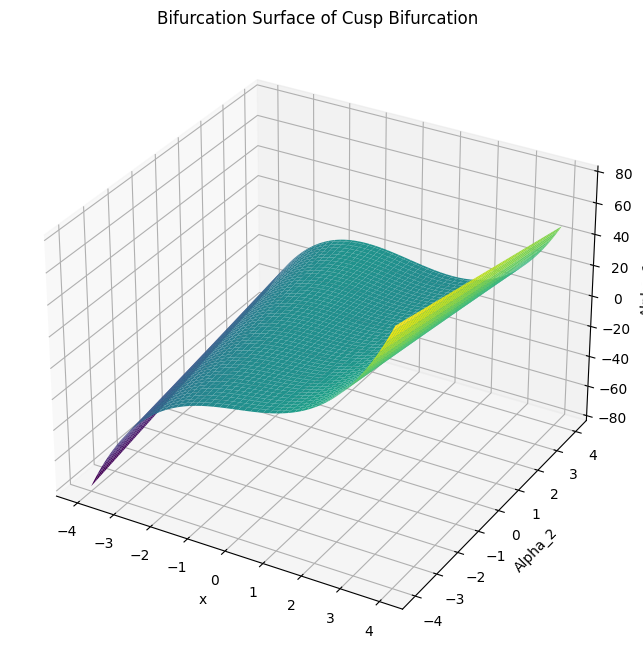
\includegraphics[width=0.45\textwidth]{images/task3/cusp-bifurcation.png}
    \caption{3D plot of the cusp bifurcation}
    \label{fig:task3_cusp-bif}
\end{figure}

% Why is it called cusp bifurcation?
As shown is the 3D plot, the name of the bifurcation must come from its characteristic shape as it highlights a sudden qualitative change in the behavior of the system. There is a sort of a threshold value of $\alpha$, really noticeable on the visualization, which marks the change. 

% Short description of the setup in the report?